\documentclass[11pt]{article}

\usepackage[margin=0.9in]{geometry}
\usepackage[T1]{fontenc}
\usepackage{newtxtext,newtxmath}
\usepackage{microtype}
\usepackage{booktabs}
\usepackage{array}
\usepackage{enumitem}
\usepackage{amsmath}
\usepackage{xcolor}
\usepackage{tikz}
\usetikzlibrary{arrows.meta,positioning,matrix,calc}
\usepackage{natbib}
\usepackage[hidelinks]{hyperref}
\usepackage{url}
\usepackage{caption}

\definecolor{accent}{HTML}{315E8A}
\definecolor{lightaccent}{HTML}{EAF1F7}
\definecolor{lightgray}{HTML}{F3F4F5}

\tikzset{
  archblock/.style={draw=black!45,rounded corners=2pt,fill=lightgray,minimum height=7.5mm,text width=18mm,align=center,inner sep=2pt,font=\scriptsize},
  archmodel/.style={draw=accent!85,rounded corners=2pt,fill=lightaccent,line width=0.9pt,minimum height=8mm,text width=19mm,align=center,inner sep=2pt,font=\scriptsize},
  archchannel/.style={draw=accent!75,rounded corners=2pt,fill=white,minimum height=7.5mm,text width=22mm,align=center,inner sep=2pt,font=\scriptsize},
  archflow/.style={-{Latex[length=1.8mm]},line width=0.65pt,draw=black!72},
  archfeedback/.style={-{Latex[length=1.7mm]},line width=0.65pt,draw=accent!80,dashed}
}

\setlength{\parindent}{1em}
\setlength{\parskip}{0pt}
\setlist{nosep,leftmargin=1.35em}
\setlength{\emergencystretch}{1.5em}
\captionsetup{font=small,skip=3pt}
\clubpenalty=10000
\widowpenalty=10000
\displaywidowpenalty=10000
\flushbottom

\newcommand{\scoretag}{\texttt{<AI SCORE: n>}}
\newcommand{\selfscore}{\textsc{SelfScore}}
\newcommand{\baseline}{\textsc{Baseline}}

\title{\vspace{-1.35em}\textbf{Inline Self-Scoring During LLM Generation}}
\author{Victor Lavrenko\\[-0.1em]
\small PeaceTech VC\\[-0.2em]
\small \texttt{victor@peacetech.vc}}
\date{October 8, 2026}

\begin{document}
\maketitle
\vspace{-1.35em}

\begin{abstract}
Many LLM systems generate an answer and evaluate it in a separate pass. We study whether self-evaluation can instead be emitted inline during the original generation trajectory, without training. Our question is deliberately prior to score calibration: if a model is already instructed to improve its output according to a criterion, does additionally requiring sentence-level self-scoring damage the generated answer? Across matched experiments covering AI-likeness, clarity, relevance, factuality, and brevity, blind evaluation shows no aggregate quality penalty from self-scoring; among directional overall-quality comparisons, self-scored outputs are preferred in 127 cases versus 92 for criterion-only generation (58.0\%). A larger AI-likeness study across 23 distinct generator model names likewise finds that inline self-scoring can coexist with generation and often improves the targeted property. Effects are heterogeneous across models and criteria, and we do not claim that the emitted scores are calibrated or useful control signals. The main result is therefore a prerequisite one: producing an inline self-evaluation channel need not degrade generation, making its calibration, training, and downstream use worth studying separately.
\end{abstract}

\section{Introduction}

Evaluation is increasingly a second inference problem: a model produces an answer, then the same or another model scores, critiques, routes, or verifies it. This enables best-of-$N$, self-correction, search, and agentic control, but requires another invocation over already-generated text. We ask a simpler architectural question: \emph{can the generator expose a local self-evaluation signal during the original trajectory without degrading the answer it is generating?}

Concurrent self-evaluation itself is not new. Most directly, \citet{zhao2024selfeval} prompted GPT-4 to emit a legal-task prediction and confidence in one call. Learned systems such as Self-RAG and confidence-token methods make reflection or confidence operational through training \citep{asai2024selfrag,chuang2025confidence}; post-hoc methods instead generate feedback and revise in later passes \citep{madaan2023selfrefine,xie2023selfevaluation}. Our narrower contribution is a generation-side test of what off-the-shelf models already do \emph{zero-shot}: repeatedly emit a local evaluation while generating, with that signal deliberately left unused downstream.

The distinction matters. Before asking whether a self-score is calibrated, predictive, or useful for branching, we first need to know whether producing it harms the primary output. We study this in two complementary ways. First, a large AI-likeness study tests four frontier models deeply and then 20 screened configurations broadly. Second, a criterion-matched study holds the optimization objective fixed and asks whether adding a score for that same objective changes overall answer quality across AI-likeness, clarity, relevance, factuality, and brevity. Figures~\ref{fig:separate-evaluation} and~\ref{fig:inline-self-scoring} show the systems motivation.

\begin{figure}[t]
\begin{minipage}[t]{0.485\linewidth}
\centering
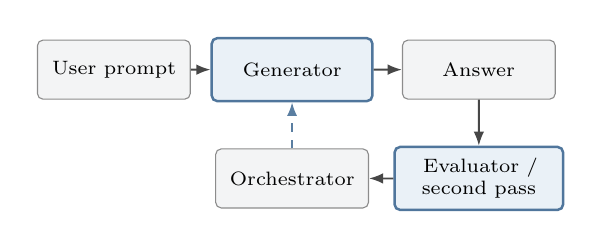
\begin{tikzpicture}[scale=0.92,transform shape]
  \matrix (m) [matrix of nodes,column sep=2.5mm,row sep=5.5mm,nodes={anchor=center},ampersand replacement=\&] {
    |[archblock]| User prompt
      \& |[archmodel]| Generator
      \& |[archblock]| Answer \\
    \& |[archblock]| Orchestrator
      \& |[archmodel,text width=20mm]| {Evaluator / second pass} \\
  };
  \draw[archflow] (m-1-1) -- (m-1-2);
  \draw[archflow] (m-1-2) -- (m-1-3);
  \draw[archflow] (m-1-3) -- (m-2-3);
  \draw[archflow] (m-2-3) -- (m-2-2);
  \draw[archfeedback] (m-2-2) -- (m-1-2);
\end{tikzpicture}
\captionof{figure}{\textbf{Separate evaluation.} A second model role or pass evaluates the answer.}
\label{fig:separate-evaluation}
\end{minipage}\hfill
\begin{minipage}[t]{0.485\linewidth}
\centering
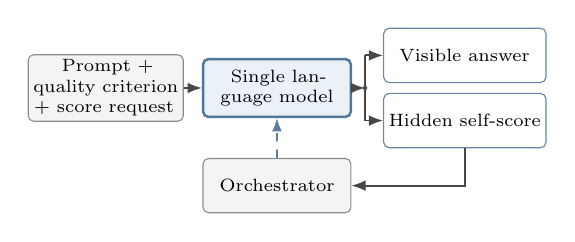
\begin{tikzpicture}[scale=0.92,transform shape,node distance=0mm]
  \node[archblock,text width=20mm] (prompt) {Prompt + quality criterion + score request};
  \node[archmodel,text width=19mm, right=2.5mm of prompt] (generator) {Single language model};
  \coordinate (fork) at ($(generator.east)+(1.8mm,0)$);
  \node[archchannel,text width=21mm, anchor=west] (answer) at ($(fork)+(2.5mm,4.5mm)$) {Visible answer};
  \node[archchannel,text width=21mm, anchor=west] (score) at ($(fork)+(2.5mm,-4.5mm)$) {Hidden self-score};
  \node[archblock,text width=19mm, below=5.5mm of generator] (orchestrator) {Orchestrator};
  \draw[archflow] (prompt) -- (generator);
  \draw[archflow] (generator.east) -- (fork);
  \fill[black!65] (fork) circle (0.9pt);
  \draw[black!72,line width=0.65pt] (fork) -- (fork |- answer.west);
  \draw[black!72,line width=0.65pt] (fork) -- (fork |- score.west);
  \draw[archflow] (fork |- answer.west) -- (answer.west);
  \draw[archflow] (fork |- score.west) -- (score.west);
  \draw[archflow] (score.south) -- ++(0,-2.5mm) |- (orchestrator.east);
  \draw[archfeedback] (orchestrator.north) -- (generator.south);
\end{tikzpicture}
\captionof{figure}{\textbf{Inline self-scoring.} One trajectory emits the answer and an evaluative side signal.}
\label{fig:inline-self-scoring}
\end{minipage}
\end{figure}

\section{Method}

\textbf{AI-likeness study.} We use 100 English prompts spanning ten domains; each requests a 5--8 sentence social-media post. Both conditions receive the same instruction to avoid generic, formulaic, clich\'ed, overly polished, promotional, repetitive, or obviously AI-generated prose. The treatment adds one requirement: after every sentence, output an integer 0--100 estimate of how AI-generated the sentence sounds, formatted as \scoretag{}. Before judging, tags are removed and whitespace normalized. Scores never trigger rejection, regeneration, branching, selection, or revision.

GPT-5.6 Sol, Claude Opus 5.5, Gemini 3.1 Pro Preview, and DeepSeek V4.1 Flash each generate both conditions for all 100 prompts: 800 accepted generations. Each cleaned pair is judged in fresh calls by all four models; the primary panel excludes the generator itself and sees both A/B orientations. The panel resolves 390/400 pairs. A breadth replication freezes 20 prompts and 20 configurations after an outcome-blind compliance screen of 24 candidates. Those configurations produce 800 generations judged by a fixed three-model external panel using the same mirrored procedure. Across the primary and breadth studies there are 23 distinct generator model names.

\textbf{Criterion-matched study.} We then test whether the generation-side result extends beyond AI-likeness. The same four generators answer 20 frozen prompts under five objectives: AI-likeness, clarity, relevance, factual accuracy, and brevity. For every generator--prompt--criterion combination, the \emph{objective-only} arm instructs the model to optimize that criterion; the \emph{self-score} arm receives the identical optimization instruction plus a 0--100 sentence-level score for that same criterion. Thus self-scoring introduces no new objective. The emitted values are stripped before evaluation and never consumed downstream. Five criteria $\times$ four models $\times$ 20 prompts $\times$ two arms yields 800 generations and 400 matched pairs; all 400 treatment outputs satisfy the frozen compliance rule.

Each pair is blindly judged in both A/B orientations by all four models. Every judge returns two decisions: \textsc{Overall}, the primary endpoint asking which answer is better for the user's task, and \textsc{Target}, asking which better satisfies the criterion being optimized. The primary external panel excludes the generator's own fresh judgment and requires at least two agreeing resolved votes. The completed run contains 3,200 mirrored judge calls. Directional rates below exclude ties and indeterminate pairs; pooled rates are descriptive because prompts, criteria, models, and developers are not independent replications.

\section{Results}

\textbf{AI-likeness at scale.} In the four-model primary study, 244 pairs favor self-scoring on the targeted AI-likeness outcome, 104 favor baseline, 42 tie, and 10 are indeterminate. Thus 70.1\% of 348 directional outcomes favor self-scoring; a prompt-cluster bootstrap gives a 95\% CI of 65.1--75.0\%. The model-level rates are 84.8\% for Claude, 75.9\% for Gemini, 68.6\% for GPT, and 49.4\% for DeepSeek.

\begin{table}[t]
\centering
\caption{AI-likeness study. Directional rates exclude ties and unresolved pairs.}
\label{tab:ailikeness}
\small
\begin{tabular}{lrrrrr}
\toprule
Generator / study & SelfScore & Baseline & Tie & Indet. & Directional \\
\midrule
Claude Opus 5.5 & 78 & 14 & 7 & 1 & 84.8\% \\
Gemini 3.1 Pro & 66 & 21 & 8 & 5 & 75.9\% \\
GPT-5.6 Sol & 59 & 27 & 14 & 0 & 68.6\% \\
DeepSeek V4.1 Flash & 41 & 42 & 13 & 4 & 49.4\% \\
\midrule
Primary total & 244 & 104 & 42 & 10 & 70.1\% \\
20-model breadth & 206 & 149 & 31 & 14 & 58.0\% \\
\bottomrule
\end{tabular}
\end{table}

The breadth effect is smaller and more heterogeneous: 206 resolved pairs favor self-scoring, 149 favor baseline, and 31 tie, so 58.0\% of 355 directional outcomes favor self-scoring. Fifteen configurations are positive, four negative, and one balanced. Related variants share developers and likely training lineage; a family/model/pair bootstrap gives 47.4--67.4\%, which includes 50\%. A strict compliance sensitivity analysis leaves the directional rate unchanged at 58.0\% (199 vs. 144, 29 ties). A 24-pair blind human pilot in a language native to the author is less decisive (7 self-score, 5 baseline, 12 ties) and does not establish a human-perceived improvement.

\textbf{Criterion-matched generation quality.} The new matched study directly tests the prerequisite claim: when the model is already instructed to optimize a property, does asking it to score that same property damage the answer? Table~\ref{tab:matched} shows that it does not produce an aggregate penalty. Across the five criteria, self-scored outputs win 127 directional overall-quality comparisons versus 92 for objective-only generation (58.0\%). The corresponding targeted-criterion count is 144 versus 83 (63.4\%).

\begin{table}[t]
\centering
\caption{Criterion-matched study. Each row compares an identical optimization objective with vs. without inline scoring of that same criterion. Rates exclude ties and indeterminate pairs.}
\label{tab:matched}
\scriptsize
\begin{tabular}{lrrr@{\hspace{1.3em}}rrr}
\toprule
& \multicolumn{3}{c}{Overall quality} & \multicolumn{3}{c}{Target criterion} \\
\cmidrule(lr){2-4}\cmidrule(lr){5-7}
Criterion & Self & Obj. & Rate & Self & Obj. & Rate \\
\midrule
AI-likeness & 42 & 15 & 73.7\% & 42 & 19 & 68.9\% \\
Clarity & 19 & 25 & 43.2\% & 24 & 17 & 58.5\% \\
Relevance & 12 & 21 & 36.4\% & 16 & 17 & 48.5\% \\
Factuality & 22 & 15 & 59.5\% & 22 & 10 & 68.8\% \\
Brevity & 32 & 16 & 66.7\% & 40 & 20 & 66.7\% \\
\midrule
Pooled, descriptive & 127 & 92 & 58.0\% & 144 & 83 & 63.4\% \\
\bottomrule
\end{tabular}
\end{table}

The result is not specific to AI-likeness, but neither is it universal. Brevity and factuality are directionally positive, clarity is weaker, and relevance does not benefit in this task set. Model heterogeneity is larger still: pooling the five criteria, overall-quality self-scoring rates are 78.4\% for GPT-5.6 Sol, 64.0\% for Claude Opus 5.5, 60.3\% for Gemini 3.1 Pro Preview, and 28.0\% for DeepSeek V4.1 Flash. The aggregate result therefore supports feasibility, not a claim that every model or criterion improves.

\section{Discussion}

The result is best interpreted as a trajectory effect, not successful self-correction. No revision occurs. After each sentence, the model makes an explicit judgment before continuing, so later tokens are conditioned on both the prose and that judgment. This could reflect prospective self-monitoring, retrospective conditioning on the emitted score, or generic extra deliberation.

The criterion-matched design sharpens the paper's main claim. The treatment does not ask the model to pursue a new goal: both arms already optimize the same property, and only one arm additionally emits a local score. Across five such objectives, requiring that score does not reduce overall answer quality in aggregate and is modestly positive descriptively. The effect's strong criterion and model dependence argues against a universal formatting trick.

This paper deliberately does \emph{not} establish that the emitted numbers are good scores. In the original AI-likeness study, mean self-scores are 14.32 when the panel later favors treatment and 14.34 when it favors baseline, so the values are not validated as ranking signals. Calibration and predictive validity are separate empirical questions. If the channel proves useful, it could subsequently be calibrated or aligned---for example through preference optimization or reinforcement learning---and used selectively for revision, branching, routing, or verification.

Relative to the closest prompt-only precedent, our contribution is therefore an extension rather than a first demonstration of concurrent self-evaluation. Zhao et al. showed that GPT-4 could emit confidence alongside a legal-task prediction; here repeated local evaluation coexists with open-ended generation across many contemporary models, and the matched study tests generation quality directly while leaving the signal unused. Learned reflection-token systems such as Self-RAG address the stronger operational problem but require training.

A practical deployment would not need to expose literal score tags to users. A model API could return the answer normally while exposing a parallel hidden control stream, as illustrated in Figure~\ref{fig:inline-self-scoring}. The present experiment does not implement that architecture; it establishes only the prerequisite that such a channel can be produced without an aggregate generation-quality penalty in the tested settings.

The main limitations are straightforward: the tasks are short explanatory prose rather than coding, mathematics, or long-form reasoning; the primary outcome is an LLM panel, and mirrored ordering mitigates but does not eliminate judge bias \citep{zheng2023judging,calderon2025alternative}; the matched generalization study uses only four generators; and closed model/provider updates complicate exact reproduction. Prior work also shows that intrinsic self-correction can fail without external feedback \citep{huang2024cannot}, so these findings should not be generalized to arbitrary correction tasks.

\section{Conclusion}

Inline self-scoring can be added to ordinary LLM generation without an aggregate loss in answer quality in the experiments reported here. In the criterion-matched study, asking models to score a property they are already instructed to optimize yields 127 overall-quality directional wins versus 92 losses across five criteria. The effect is not limited to AI-likeness, although both criterion and model matter substantially. A larger AI-likeness study across 23 distinct generator names likewise shows that the act of inline self-evaluation can alter the generated output, often beneficially.

These results do not establish that zero-shot self-scores are calibrated evaluators or useful control signals. They establish the earlier prerequisite: producing an inline evaluation channel need not damage the primary output. This makes the quality, training, calibration, and downstream use of that channel a meaningful next question.

\section*{Reproducibility and AI Assistance}

The reproducibility package contains frozen prompts, provider pins, raw generations and mirrored judgments, compliance screening, SQLite logs, analyses, and human-validation materials; it is available at \url{https://github.com/victorlavrenko/llm-inline-self-scoring}. OpenAI ChatGPT (GPT-5.6 Sol) assisted with code organization, literature discovery, statistical cross-checking, drafting, editing, and LaTeX preparation. The author designed and ran the experiments, verified the results and references, and takes responsibility for all claims.

\clearpage
\bibliographystyle{plainnat}
\bibliography{refs}

\end{document}
